\documentclass{standalone}
\usepackage{tikz}
\usetikzlibrary{patterns, positioning}


\begin{document}
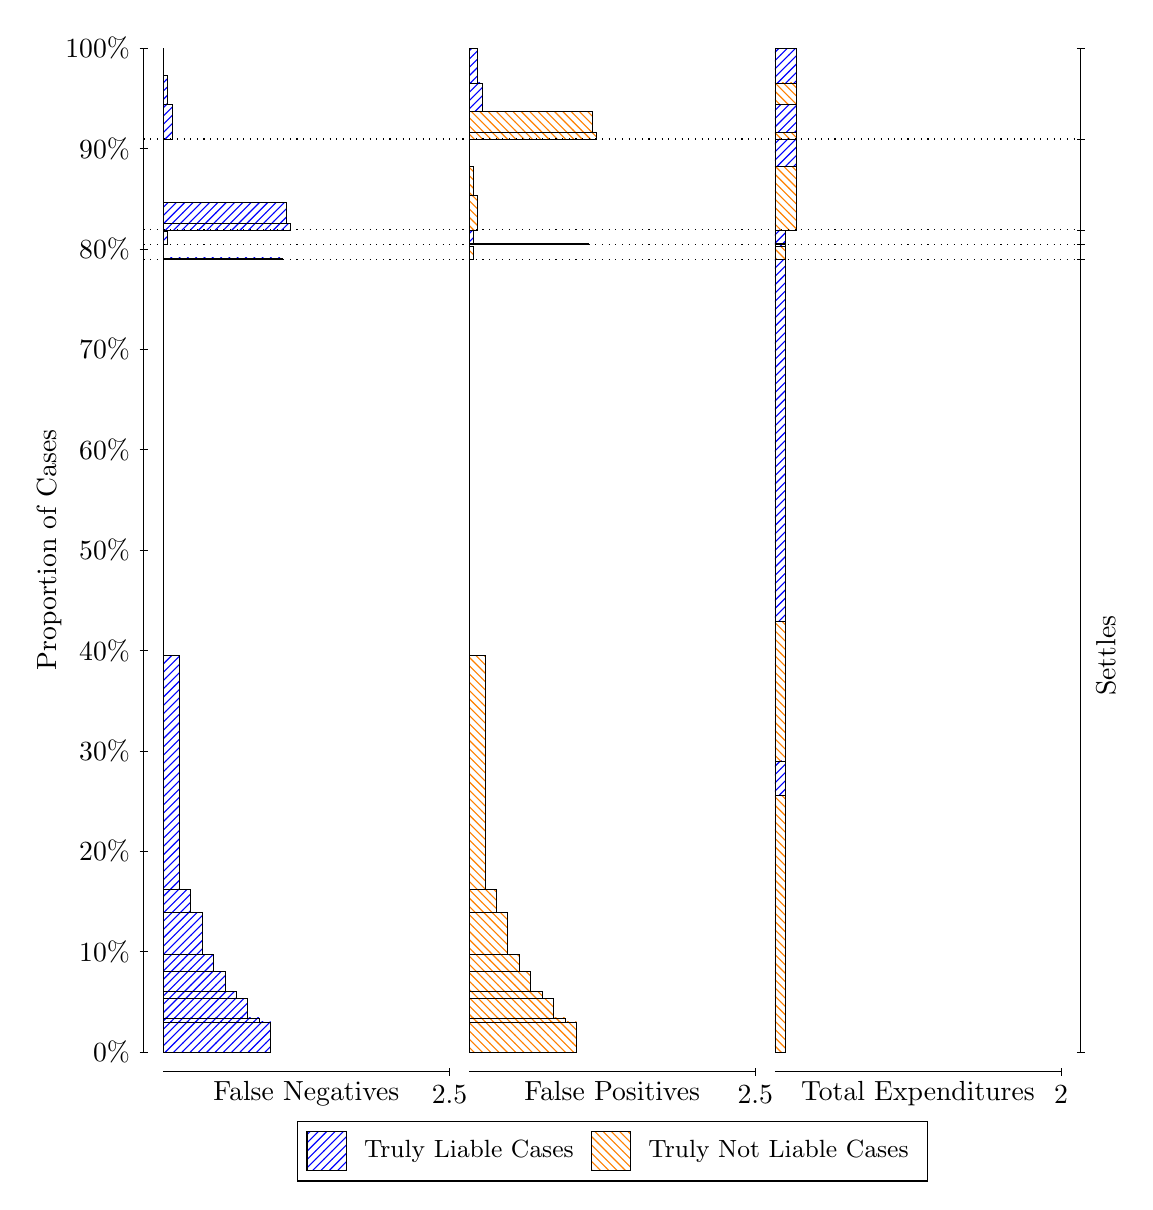
\begin{tikzpicture}
\draw[black, very thin] (1.5,1.75) -- (1.5,14.5);
\node[rotate=90, text=black, anchor=center] at (0.3, 8.125) {Proportion of Cases};
\draw[black, very thin] (1.45,1.75) -- (1.55,1.75);
\node[text=black, anchor=east] at (1.45, 1.75) {0\%};
\draw[black, very thin] (1.45,3.025) -- (1.55,3.025);
\node[text=black, anchor=east] at (1.45, 3.025) {10\%};
\draw[black, very thin] (1.45,4.3) -- (1.55,4.3);
\node[text=black, anchor=east] at (1.45, 4.3) {20\%};
\draw[black, very thin] (1.45,5.575) -- (1.55,5.575);
\node[text=black, anchor=east] at (1.45, 5.575) {30\%};
\draw[black, very thin] (1.45,6.85) -- (1.55,6.85);
\node[text=black, anchor=east] at (1.45, 6.85) {40\%};
\draw[black, very thin] (1.45,8.125) -- (1.55,8.125);
\node[text=black, anchor=east] at (1.45, 8.125) {50\%};
\draw[black, very thin] (1.45,9.4) -- (1.55,9.4);
\node[text=black, anchor=east] at (1.45, 9.4) {60\%};
\draw[black, very thin] (1.45,10.675) -- (1.55,10.675);
\node[text=black, anchor=east] at (1.45, 10.675) {70\%};
\draw[black, very thin] (1.45,11.95) -- (1.55,11.95);
\node[text=black, anchor=east] at (1.45, 11.95) {80\%};
\draw[black, very thin] (1.45,13.225) -- (1.55,13.225);
\node[text=black, anchor=east] at (1.45, 13.225) {90\%};
\draw[black, very thin] (1.45,14.5) -- (1.55,14.5);
\node[text=black, anchor=east] at (1.45, 14.5) {100\%};

\draw[black, very thin] (13.4,1.75) -- (13.4,14.5);
\draw[black, very thin] (13.35,1.75) -- (13.45,1.75);
\node[anchor=west] at (13.35, 1.75) {};
\draw[black, very thin] (13.35,11.815) -- (13.45,11.815);
\node[anchor=west] at (13.35, 11.815) {};
\draw[black, very thin] (13.35,12.002) -- (13.45,12.002);
\node[anchor=west] at (13.35, 12.002) {};
\draw[black, very thin] (13.35,12.19) -- (13.45,12.19);
\node[anchor=west] at (13.35, 12.19) {};
\draw[black, very thin] (13.35,13.345) -- (13.45,13.345);
\node[anchor=west] at (13.35, 13.345) {};
\draw[black, very thin] (13.35,14.5) -- (13.45,14.5);
\node[anchor=west] at (13.35, 14.5) {};

\draw[black, very thin, pattern color=blue, pattern=north east lines] (1.75,1.75) rectangle (3.1125,2.1313);
\draw[black, very thin, pattern color=blue, pattern=north east lines] (1.75,2.1313) rectangle (2.9672,2.1842);
\draw[black, very thin, pattern color=blue, pattern=north east lines] (1.75,2.1842) rectangle (2.8218,2.4266);
\draw[black, very thin, pattern color=blue, pattern=north east lines] (1.75,2.4266) rectangle (2.6765,2.5188);
\draw[black, very thin, pattern color=blue, pattern=north east lines] (1.75,2.5188) rectangle (2.5312,2.7767);
\draw[black, very thin, pattern color=blue, pattern=north east lines] (1.75,2.7767) rectangle (2.3858,2.9895);
\draw[black, very thin, pattern color=blue, pattern=north east lines] (1.75,2.9895) rectangle (2.2405,3.5195);
\draw[black, very thin, pattern color=blue, pattern=north east lines] (1.75,3.5195) rectangle (2.0952,3.8153);
\draw[black, very thin, pattern color=blue, pattern=north east lines] (1.75,3.8153) rectangle (1.9498,6.7822);
\draw[black, very thin, pattern color=orange, pattern=north west lines] (1.75,6.7822) rectangle (1.75,11.815);
\draw[black, very thin, pattern color=blue, pattern=north east lines] (1.75,11.815) rectangle (3.2578,11.835);
\draw[black, very thin, pattern color=orange, pattern=north west lines] (1.75,11.835) rectangle (1.75,12.002);
\draw[black, very thin, pattern color=blue, pattern=north east lines] (1.75,12.002) rectangle (1.8045,12.169);
\draw[black, very thin, pattern color=orange, pattern=north west lines] (1.75,12.169) rectangle (1.75,12.19);
\draw[black, very thin, pattern color=blue, pattern=north east lines] (1.75,12.19) rectangle (3.3668,12.272);
\draw[black, very thin, pattern color=blue, pattern=north east lines] (1.75,12.272) rectangle (3.3123,12.541);
\draw[black, very thin, pattern color=orange, pattern=north west lines] (1.75,12.541) rectangle (1.75,13.345);
\draw[black, very thin, pattern color=blue, pattern=north east lines] (1.75,13.345) rectangle (1.859,13.789);
\draw[black, very thin, pattern color=blue, pattern=north east lines] (1.75,13.789) rectangle (1.8045,14.149);
\draw[black, very thin, pattern color=orange, pattern=north west lines] (1.75,14.149) rectangle (1.75,14.5);
\draw[black, very thin, pattern color=orange, pattern=north west lines] (5.6333,1.75) rectangle (6.9958,2.1313);
\draw[black, very thin, pattern color=orange, pattern=north west lines] (5.6333,2.1313) rectangle (6.8505,2.1842);
\draw[black, very thin, pattern color=orange, pattern=north west lines] (5.6333,2.1842) rectangle (6.7052,2.4266);
\draw[black, very thin, pattern color=orange, pattern=north west lines] (5.6333,2.4266) rectangle (6.5598,2.5188);
\draw[black, very thin, pattern color=orange, pattern=north west lines] (5.6333,2.5188) rectangle (6.4145,2.7767);
\draw[black, very thin, pattern color=orange, pattern=north west lines] (5.6333,2.7767) rectangle (6.2692,2.9895);
\draw[black, very thin, pattern color=orange, pattern=north west lines] (5.6333,2.9895) rectangle (6.1238,3.5196);
\draw[black, very thin, pattern color=orange, pattern=north west lines] (5.6333,3.5196) rectangle (5.9785,3.8153);
\draw[black, very thin, pattern color=orange, pattern=north west lines] (5.6333,3.8153) rectangle (5.8332,6.7824);
\draw[black, very thin, pattern color=blue, pattern=north east lines] (5.6333,6.7824) rectangle (5.6333,11.815);
\draw[black, very thin, pattern color=orange, pattern=north west lines] (5.6333,11.815) rectangle (5.6878,11.981);
\draw[black, very thin, pattern color=blue, pattern=north east lines] (5.6333,11.981) rectangle (5.6333,12.002);
\draw[black, very thin, pattern color=orange, pattern=north west lines] (5.6333,12.002) rectangle (7.1412,12.023);
\draw[black, very thin, pattern color=blue, pattern=north east lines] (5.6333,12.023) rectangle (5.6878,12.19);
\draw[black, very thin, pattern color=orange, pattern=north west lines] (5.6333,12.19) rectangle (5.7423,12.634);
\draw[black, very thin, pattern color=orange, pattern=north west lines] (5.6333,12.634) rectangle (5.6878,12.994);
\draw[black, very thin, pattern color=blue, pattern=north east lines] (5.6333,12.994) rectangle (5.6333,13.345);
\draw[black, very thin, pattern color=orange, pattern=north west lines] (5.6333,13.345) rectangle (7.2502,13.427);
\draw[black, very thin, pattern color=orange, pattern=north west lines] (5.6333,13.427) rectangle (7.1957,13.696);
\draw[black, very thin, pattern color=blue, pattern=north east lines] (5.6333,13.696) rectangle (5.7968,14.056);
\draw[black, very thin, pattern color=blue, pattern=north east lines] (5.6333,14.056) rectangle (5.7423,14.5);
\draw[black, very thin, pattern color=orange, pattern=north west lines] (9.5167,1.75) rectangle (9.6529,5.0128);
\draw[black, very thin, pattern color=blue, pattern=north east lines] (9.5167,5.0128) rectangle (9.6529,5.447);
\draw[black, very thin, pattern color=orange, pattern=north west lines] (9.5167,5.447) rectangle (9.6529,7.2165);
\draw[black, very thin, pattern color=blue, pattern=north east lines] (9.5167,7.2165) rectangle (9.6529,11.815);
\draw[black, very thin, pattern color=orange, pattern=north west lines] (9.5167,11.815) rectangle (9.6529,11.981);
\draw[black, very thin, pattern color=blue, pattern=north east lines] (9.5167,11.981) rectangle (9.6529,12.002);
\draw[black, very thin, pattern color=orange, pattern=north west lines] (9.5167,12.002) rectangle (9.6529,12.023);
\draw[black, very thin, pattern color=blue, pattern=north east lines] (9.5167,12.023) rectangle (9.6529,12.19);
\draw[black, very thin, pattern color=orange, pattern=north west lines] (9.5167,12.19) rectangle (9.7892,12.994);
\draw[black, very thin, pattern color=blue, pattern=north east lines] (9.5167,12.994) rectangle (9.7892,13.345);
\draw[black, very thin, pattern color=orange, pattern=north west lines] (9.5167,13.345) rectangle (9.7892,13.427);
\draw[black, very thin, pattern color=blue, pattern=north east lines] (9.5167,13.427) rectangle (9.7892,13.787);
\draw[black, very thin, pattern color=orange, pattern=north west lines] (9.5167,13.787) rectangle (9.7892,14.056);
\draw[black, very thin, pattern color=blue, pattern=north east lines] (9.5167,14.056) rectangle (9.7892,14.5);
\draw[black, dotted] (1.5,11.815) -- (13.4,11.815);
\draw[black, dotted] (1.5,12.002) -- (13.4,12.002);
\draw[black, dotted] (1.5,12.19) -- (13.4,12.19);
\draw[black, dotted] (1.5,13.345) -- (13.4,13.345);
\draw[black, very thin] (1.75,1.5) -- (5.3833,1.5);
\node[text=black, anchor=north] at (3.5667, 1.5) {False Negatives};
\draw[black, very thin] (5.3833,1.45) -- (5.3833,1.55);
\node[text=black, anchor=north] at (5.3833, 1.45) {2.5};

\draw[black, very thin] (5.6333,1.5) -- (9.2667,1.5);
\node[text=black, anchor=north] at (7.45, 1.5) {False Positives};
\draw[black, very thin] (9.2667,1.45) -- (9.2667,1.55);
\node[text=black, anchor=north] at (9.2667, 1.45) {2.5};

\draw[black, very thin] (9.5167,1.5) -- (13.15,1.5);
\node[text=black, anchor=north] at (11.333, 1.5) {Total Expenditures};
\draw[black, very thin] (13.15,1.45) -- (13.15,1.55);
\node[text=black, anchor=north] at (13.15, 1.45) {2};

\node[text=black, centered, rotate=90] at (13.72, 6.7823) {Settles};





\draw (7.449999999999999,1.5) node[draw=none] (baseCoordinate) {};
\begin{scope}[align=center]
        \matrix[scale=0.5, draw=black, below=0.5cm of baseCoordinate, nodes={draw}, column sep=0.1cm]{
            \node[rectangle, draw, minimum width=0.5cm, minimum height=0.5cm, pattern color=blue, pattern=north east lines] {}; &
            \node[draw=none, font=\small, text=black] (B) {Truly Liable Cases}; &
            \node[rectangle, draw, minimum width=0.5cm, minimum height=0.5cm, pattern color=orange, pattern=north west lines] {}; &
            \node[draw=none, font=\small, text=black] (B) {Truly Not Liable Cases}; \\
            };
\end{scope}

\end{tikzpicture}
\end{document}